\documentclass[a4paper]{report}
\usepackage{longtable,float,hyperref,color,amsmath,amsxtra,amssymb,latexsym,amscd,amsthm,amsfonts,graphicx,enumitem,parskip,imakeidx,soul}
\usepackage{tikz,graphicx}
\usetikzlibrary{shapes,arrows}
\usetikzlibrary{calc}
\usetikzlibrary{decorations.pathreplacing,angles,quotes}
%\numberwithin{equation}{section}
%\allowdisplaybreaks
%\usepackage{fancyhdr}
%\pagestyle{fancy}
%\fancyhf{}
%\fancyhead[RE,LO]{\footnotesize \textsc \leftmark}
%\cfoot{\thepage}
%\renewcommand{\headrulewidth}{0.5pt}
%\setcounter{tocdepth}{1}
%\setcounter{secnumdepth}{1}
\usepackage[utf8x]{inputenc}
%\usepackage[utf8x]{vietnam}    
%\setlength\parindent{0pt}
\makeindex[columns=2, title=Alphabetical Index, 
           options= -s index.ist]
\title{\Huge Homework Assignment\\Differential Geometry}
\author{\textsc{Doan Tran Nguyen Tung}\\
{\small \texttt{Student ID: 1411352}}}

\DeclareMathOperator{\const}{const}
\makeatletter
\DeclareMathOperator{\trace}{trace}
\makeatletter
\DeclareMathOperator{\arsech}{arsech}
\makeatletter
\DeclareMathOperator{\arcsch}{arcsch}
\makeatletter
\DeclareMathOperator{\arcosh}{arcosh}
\makeatletter
\DeclareMathOperator{\arsinh}{arsinhh}
\makeatletter

\begin{document}
\maketitle
\textbf{Exercise 5} (p.168, \cite{2}) Consider the parametrized surface (Enneper's surface)
\begin{align}
	x(u,v) = \left(u - \frac{u^3}{3} + u v^2, v - \frac{v^3}{3} + v u^2, u^2 - v^2\right)
\end{align}
and show that
\begin{enumerate}[label=\textbf{(\alph*)}, leftmargin=*]
	\item\label{5a} The coefficients of the first fundamental form are
	\begin{align}
		E = G = (1+u^2 + v^2)^2, \enskip F = 0
	\end{align}
	\item\label{5b} The coefficients of the second fundamental form are
	\begin{align}
		e = 2, \enskip g = -2, \enskip f = 0
	\end{align}
	\item\label{5c} The principal curvatures are 
	\begin{align}
		k_1 = \frac{2}{(1+u^2+v^2)^2}, \enskip k_2 = -\frac{2}{(1+u^2+v^2)^2}
	\end{align}
	\item\label{5d} The lines of curvature are the coordinate curves. 
	\item\label{5e} The asymptotic curves are $u+v= \const$, $u - v = \const$
\end{enumerate}
\textsc{Solution} 

\ref{5a} We have
\begin{align}
	x_u(u,v) &= \left(1 - u^2 + v^2, 2vu, 2u \right)\\
	x_v(u,v) &= \left(2uv, 1 - v^2 + u^2, -2v \right)
\end{align}
Using these, we can compute the coefficient of the first fundamental form
\begin{align}
	E &= \langle x_u, x_u \rangle\\
	&= (1 - u^2 + v^2)^2 + 4v^2u^2 + 4u^2 \\
	&= (u^4 - 2u^2v^2 - 2u^2 + v^4 + 2v^2 + 1) + 4v^2u^2 + 4u^2\\
	&= (u^4 + 2u^2v^2 + 2u^2 + v^4 + 2v^2 + 1) \\
	&= (1+u^2 + v^2)^2\\
	F &= \langle x_u, x_v \rangle \\
	&= (1 - u^2 + v^2)2uv + 2vu(1 - v^2 + u^2) - 4uv\\
	&= 2uv - 2u^3v + 2uv^3 + 2vu - 2v^3u + 2vu^3 - 4uv\\
	&= 0 \\
	G &= \langle x_v, x_v \rangle \\
	&= 4u^2v^2 + (1 - v^2 + u^2)^2 + 4v^2\\
	&= (u^4 - 2u^2v^2 + 2u^2 + v^4 - 2v^2 + 1) + 4u^2v^2 + 4v^2\\
	&= (u^4 + 2u^2v^2 + 2u^2 + v^4 + 2v^2 + 1) \\
	&= (1+u^2 + v^2)^2
\end{align}

\ref{5b} The unit normal vector at $x(u,v)$ is define as
\begin{align}
	\nu(u,v) &= N(x(u,v))\\
	&= \frac{x_u \times x_v}{\lVert x_u \times x_v \rVert}\\
	&= \frac{\left(-2u^3 - 2uv^2 - 2u, 2v^3 + 2vu^2 + 2v, - u^4 - 2u^2v^2 - v^4 + 1 \right)}{\sqrt{(-2u^3 - 2uv^2 - 2u)^2 + (2v^3 + 2vu^2 + 2v)^2 + (- u^4 - 2u^2v^2 - v^4 + 1)^2}}\\
	&= \frac{\left(-2u^3 - 2uv^2 - 2u, 2v^3 + 2vu^2 + 2v, - u^4 - 2u^2v^2 - v^4 + 1 \right)}{(1 + u^2 + v^2)^2}
\end{align}
The second order partial derivative of $x$ can be computed as
\begin{align}
	x_{u,u}(u,v) &= \left(-2u, 2v, 2 \right)\\
	x_{u,v}(u,v) &= \left(2v, 2u, 0 \right)\\
	x_{v,v}(u,v) &= \left(2u, -2v, -2 \right) = - x_{u,u}(u,v)
\end{align}
Hence, the coefficients of the second fundamental form are
\begin{align}
	e &= \langle \nu, x_{u,u} \rangle\\
	&= \frac{-2u(-2u^3 - 2uv^2 - 2u) + 2v(2v^3 + 2vu^2 + 2v) + 2(- u^4 - 2u^2v^2 - v^4 + 1)}{(1 + u^2 + v^2)^2}\\
	&= 2\frac{2u^4 + 2u^2v^2 + 2u^2 + 2v^4 + 2v^2u^2 + 2v^2 - u^4 - 2u^2v^2 - v^4 + 1}{(1 + u^2 + v^2)^2}\\
	&= 2\frac{u^4 + 2u^2v^2 + 2u^2 + v^4 + 2v^2 + 1}{(1 + u^2 + v^2)^2}\\
	&= 2\frac{(1 + u^2 + v^2)^2}{(1 + u^2 + v^2)^2}\\
	&= 2\\
	f &= \langle \nu, x_{u,v} \rangle \\
	&= \frac{2u(-2u^3 - 2uv^2 - 2u) + 2v(2v^3 + 2vu^2 + 2v)}{(1 + u^2 + v^2)^2}\\
	&=\frac{(-4u^4 - 4u^2v^2 - 4u^2) + (4v^4 + 4v^2u^2 + 4v^2)}{(1 + u^2 + v^2)^2}\\
	&=\frac{0}{(1 + u^2 + v^2)^2}\\
	&= 0 \\
	g &= \langle \nu, x_{v,v} \rangle \\
	&= -\langle \nu, x_{u,u} \rangle \\
	&= -2
\end{align}

\ref{5c}

The Gaussian curvature can be computed as
\begin{align}
	K = k_1 k_2 &= \left\lvert \left[\begin{array}{cc}
	e & f \\ 
	f & g
	\end{array} \right] \left[\begin{array}{cc}
	E & F \\ 
	F & G
	\end{array} \right]^{-1} \right\rvert\\
	&= \frac{\left\lvert \left[\begin{array}{cc}
		e & f \\ 
		f & g
		\end{array} \right] \right\rvert}{\left\lvert \left[\begin{array}{cc}
		E & F \\ 
		F & G
		\end{array} \right] \right\rvert}\\
	&= \frac{eg - f^2}{EG - F^2}
\end{align}
The mean curvature can be computed as
\begin{align}
	H = \frac{k_1 + k_2}{2} &= \frac{1}{2}\trace\left( \left[\begin{array}{cc}
	e & f \\ 
	f & g
	\end{array} \right] \left[\begin{array}{cc}
	E & F \\ 
	F & G
	\end{array} \right]^{-1}\right)\\
	&= \frac{1}{2} \trace\left( \frac{1}{EG - F^2} \left[\begin{array}{cc}
	Ge - Ff & Ef - Fe \\ 
	Gf - Fg & Eg - Ff
	\end{array} \right] \right)\\
	&= \frac{1}{2} \frac{Ge - 2Ff + Eg}{EG - F^2}\\
\end{align}
Hence, we have
\begin{align}
&\begin{cases}
k_1 k_2 &= K\\
k_1 + k_2 &= 2H
\end{cases}\\
\Leftrightarrow &
\begin{cases}
k_1 (2H - k_1) &= K\\
k_2 &= 2H - k_1
\end{cases}\\
\Leftrightarrow &
\begin{cases}
- k_1^2 + 2Hk_1 &= K\\
k_2 &= 2H - k_1
\end{cases}\\
\Leftrightarrow &
\begin{cases}
k_1^2 - 2Hk_1 + K &= 0\\
k_2 &= 2H - k_1
\end{cases}\\
\Leftrightarrow &
\begin{cases}
k_1 &= H - \sqrt{H^2 - K} \enskip \mbox{ or }\enskip k_1 = H + \sqrt{H^2 - K}\\
k_2 &= 2H - k_1 
\end{cases}
\end{align}
Since $2H - (H + \sqrt{H^2 - K} )  = H - \sqrt{H^2 - K}$, we can choose
\begin{align}
	\begin{cases}
	k_1 &= H + \sqrt{H^2 - K}\\
	k_2 &= H - \sqrt{H^2 - K}
	\end{cases}
\end{align}
We have
\begin{align}
	H^2 - K =& \frac{1}{4} \frac{(Ge - 2Ff + Eg)^2}{(EG - F^2)^2} - \frac{eg - f^2}{EG - F^2}\\
	=& \frac{1}{4} \frac{(Ge - 2Ff + Eg)^2}{(EG - F^2)^2} - \frac{(eg - f^2)(EG - F^2)}{(EG - F^2)^2}\\
	=& \frac{1}{4} \frac{E^2g^2 - 4EFfg + 2EGeg + 4F^2f^2 - 4FGef + G^2e^2}{(EG - F^2)^2}\\
	&- \frac{1}{4} 4\frac{F^2f^2 - egF^2 - EGf^2 + EGeg}{(EG - F^2)^2}\\
	=& \frac{1}{4} \frac{E^2g^2 - 4EFfg + 2EGeg + 4F^2f^2 - 4FGef + G^2e^2}{(EG - F^2)^2}\\
	&+ \frac{1}{4} \frac{-4F^2f^2 + 4egF^2 + 4EGf^2 - 4EGeg}{(EG - F^2)^2}\\
	=& \frac{1}{4} \frac{E^2g^2 - 4EFfg - 2EGeg + 4EGf^2 + 4F^2eg - 4FGef + G^2e^2}{(EG - F^2)^2}\\
\end{align}
Since $F = f = 0$,
\begin{align}
	H &= \frac{1}{2} \frac{Ge + Eg}{EG}
\end{align}
\begin{align}
	H^2 - K &= \frac{1}{4} \frac{E^2g^2 - 2EGeg + G^2e^2}{(EG)^2}\\
	&= \frac{1}{4} \frac{(Eg - Ge)^2}{(EG)^2}
\end{align}
Then, we have
\begin{align}
\begin{cases}
k_1 &= H + \sqrt{H^2 - K} = \dfrac{1}{2} \dfrac{Ge + Eg}{EG} + \dfrac{1}{2} \left \lvert\dfrac{Eg - Ge}{EG}\right\rvert\\
k_2 &= H - \sqrt{H^2 - K} =\dfrac{1}{2} \dfrac{Ge + Eg}{EG} - \dfrac{1}{2} \left \lvert\dfrac{Eg - Ge}{EG}\right\rvert
\end{cases}
\end{align}
We can choose
\begin{align}
\begin{cases}
k_1 &= \dfrac{1}{2} \dfrac{Ge + Eg}{EG} - \dfrac{1}{2}\dfrac{Eg - Ge}{EG} = \dfrac{Ge}{EG} = \dfrac{e}{E} = \dfrac{2}{(1 + u^2 + v^2)^2}\\
k_2 &= \dfrac{1}{2} \dfrac{Ge + Eg}{EG} + \dfrac{1}{2}\dfrac{Eg - Ge}{EG} = \dfrac{Eg}{EG} = \dfrac{g}{G} = \dfrac{-2}{(1 + u^2 + v^2)^2}
\end{cases}
\end{align}

\newpage
\ref{5d}

According to p.161, \cite{2}, a connected regular curve $C$ in the coordinate neighborhood of $x$ is a line of curvature if and only if for any parametrization $\alpha(t) = x(u(t), v(t))$, $t \in I$ of $C$, we have
\begin{align}
	dN(\alpha'(t)) = \lambda(t) \alpha'(t)
\end{align}
It follows that $u'(t)$ and $v'(t)$ satisfy the differential equation of the lines of curvature
\begin{align}
	\label{deloc}
	(fE − eF)(u′)^2 + (gE − eG)u′v′ + (gF − fG)(v′)^2 = 0
\end{align}
In our case, \eqref{deloc} is
\begin{align}
	-2(1+u^2+v^2)u'v' - 2(1+u^2+v^2)u'v' =0
\end{align}
or
\begin{align}
	\label{deloc_1}
	(1+u^2+v^2)u'v' =0
\end{align}
Since $1+u^2+v^2 > 0$, this implies that either $u' = 0$ or $v' = 0$, which means either $u(t)$ or $v(t)$ must be invariant as $t$ change. In other words, $C$ must be a coordinate curve.

Therefore, the lines of curvature are the coordinate curves.

\ref{5e}

According to p.160, \cite{2}, a connected regular curve $C$ in the coordinate neighborhood of $x$ is an asymptotic curve if and only if for any parametrization $\alpha(t) = x(u(t), v(t))$, $t \in I$ of $C$, we have $II(\alpha'(t)) = 0$, for all $t \in I$, that is, if and only if $u'$ and $v'$ satisfy the differential equation of the asymptotic curves
\begin{align}
	\label{deac}
	e(u′)^2 + 2fu′v′ + g(v′)^2 = 0
\end{align}
In our case, \eqref{deac} is
\begin{align}
2(u′)^2 - 2(v′)^2 = 0
\end{align}
or
\begin{align}
	\label{deac_1}
	(u′)^2 = (v′)^2
\end{align}
which means that
\begin{align}
	u' = v' \enskip\mbox{ or }\enskip u' = -v'
\end{align}
Integrating both sides, we have
\begin{align}
	u = v + \const \enskip\mbox{ or }\enskip u = -v + \const
\end{align}
This is equivalent to
\begin{align}
	u - v = \const \enskip\mbox{ or }\enskip u + v = \const
\end{align}
Therefore, the asymptotic curves are $u+v= \const$, $u - v = \const$.

\newpage
\textbf{Exercise 6} (p.168, \cite{2}) (A surface with $K = -1$, the Pseudosphere)
\begin{enumerate}[label=\textbf{(\alph*)}, leftmargin=*]
	\item\label{6a} Determine an equation for the plane curve $C$, which is such that the segment of the tangent line between the point of tangency and some line $r$ in the plane, which does not meet the curve, is constantly equal to $1$ (this curve is called the tractrix). 
	\item\label{6b} Rotate the tractrix $C$ about the line $r$; determine if the "surface" of revolution thus obtained (the pseudosphere) is regular and find out a parametrization in a neighborhood of a regular point. 
	\item\label{6c} Show that the Gaussian curvature of any regular point of the pseudosphere is $-1$.
\end{enumerate}
\textsc{Solution} 

\ref{6a} Let $r$ be some line in a plane, with out loss of generality, we can choose the Cartesian coordinates such that the z-axis coincides with $r$ and $xOz$ is the plane where $r$ is in.

Let $C(x) = (x,f(x))$ be a parameterization of a curve $C$ in the plane $xOz$. Suppose that $(a,f(a))$ is a point on $C$, the tangent line of $C$ at $(a,f(a))$ (denoted by $T_{C,a}(x,z)$) is given by
\begin{align}
	z = f(a) + f'(a)(x-a)
\end{align}
where $f'(a) = \dfrac{df}{dx}(a)$.

Let $(0,b)$ be the intersection of $T_{C,a}$ and the z-axis, $b$ is given by
\begin{align}
	b &= f(a) + f'(a)(0-a)\\
	&= f(a) - af'(a)
\end{align}
The distance between $(a,f(a))$ and $(0,b)$ is
\begin{align}
	\sqrt{\left(a - 0\right)^2 + \left(f(a) - b\right)^2} &= \sqrt{a^2 + \left(f(a) - f(a) + af'(a)\right)^2}\\
	 &= \sqrt{a^2 + a^2{f'}^2(a)}\\
\end{align}
Then, if the distance between $(a,f(a))$ and $(0,b)$ is constantly equal to $1$, we have the equation
\begin{align}
	\sqrt{a^2 + a^2{f'}^2(a)} &= 1
\end{align}
or
\begin{align}
{f'}^2(a) &= \frac{1 - a^2}{a^2} \label{6a_eq0}
\end{align}
with the condition $0<\lvert a \rvert \leq 1$.

Assume that $C$ is completely on the right side of $Oz$, using \eqref{6a_eq0}, we can find an equation for $f$ by pluging $x\in (0,1]$ into $a$,
\begin{align}
	{f'}^2(x) &= \frac{1 - x^2}{x^2} \label{6a_eq1}
\end{align}
With \eqref{6a_eq1}, we note that $C$ can be interpreted as an union of $2$ curves, given respectively by the parameterization $C_1(x)=(x,f_1(x))$ and $C_2(x)=(x,f_2(x))$ where
\begin{align}
	f_1'(x) &= \frac{\sqrt{1 - x^2}}{x} \label{6a_f11}\\
	f_2'(x) &= -\frac{\sqrt{1 - x^2}}{x}\label{6a_f21}
\end{align}
We notice that $f_1'$ and $f_2'$ coincide at $x = 1$ and we will not be able to determine the curve $C$ using only the above differential equations, since those equations only give us the shape of the curve but not the position.

Therefore, we must specify a condition to constrain the position of $C$ in the plane, in this this case, we can choose the condition $C(1) = (1,f(1)) = (1,0)$, or $f_1(1) = f_2(1) = 0$.

Consider the initial value problem
\begin{align}
	\begin{cases}
	f_1'(x) &= \dfrac{\sqrt{1 - x^2}}{x}\\
	f_1(1) &= 0
	\end{cases}
\end{align}
Using the Newton–Leibniz formula, integrating both sides of \eqref{6a_f11} yields
\begin{align}
	f_1(x) &= \int_{1}^{x} \frac{\sqrt{1 - \bar{x}^2}}{\bar{x}} d\bar{x} + f_1(1)\\
	&= \left(\sqrt{1 - x^2} - \ln\frac{1 + \sqrt{1 - x^2}}{x}\right) + 0\\
	&= \sqrt{1 - x^2} - \ln\frac{1 + \sqrt{1 - x^2}}{x}\\
	&= \sqrt{1 - x^2} - \arsech x \label{6a_f1}
\end{align}
Similarly, integrating both sides of \eqref{6a_f21} yields
\begin{align}
f_2(x) &= \ln\frac{1 + \sqrt{1 - x^2}}{x} - \sqrt{1 - x^2}\\
&= \arsech x - \sqrt{1 - x^2}\\
&= - f_1(x)\label{6a_f2}
\end{align}
where $\arsech$ is the inverse hyperbolic secant function given by
\begin{align}
	\arsech x = \ln\frac{1 + \sqrt{1 - x^2}}{x}
\end{align}
with the derivative
\begin{align}
	\arsech' x = \frac{d}{dx} \arsech x = \frac{-1}{x\sqrt{1 - x^2}}
\end{align}
By \eqref{6a_f1}, \eqref{6a_f2} and the initial condition $f_1(1) = f_2(1) = 0$, we can see that $C_1$ and $C_2$ is symmetric about the x-axis.

Thus, for many purpose, we can evaluate the properties of the $C_1$ part of the curve $C$ and deduce the properties of the rest using the property of symmetry.

\newpage
\ref{6b} Let $C$ be the generating curve for the surface of revolution $S_C$ obtained by rotating $C$ around the z-axis.

Since $C$ is the union of two curve $C_1$ and $C_2$, which are symmetric about the x-axis, we consider partitioning $S_C$ into 3 parts $S_{C_1}$, $S_{C_2}$ and $S_{C_0}$ as follows

$\bullet$ \textbf{Part 1:} $S_{C_1}$ is the surface of revolution obtained by rotating the curve $C_1$ minus $C_1(1)=(1,0)$ around the z-axis

$\bullet$ \textbf{Part 2:} $S_{C_2}$ is the surface of revolution obtained by rotating the curve $C_2$ minus $C_2(1)=(1,0)$ around the z-axis

$\bullet$ \textbf{Part 3:} $S_{C_0}$ is the surface of revolution obtained by rotating the curve $C_0 = C_1 \cap C_2$. Actually, $C_0$ is the point $(1,0)$ on the $xOz$ plane. In other words $S_{C_0}$ is the circle on the plane $xOy$ with radius $1$ and center at $O$.

Firstly, we consider a local parameterization of $S_{C_1}$
\begin{align}
	X_1(u,v) = \left(\varphi(v) \cos u, \varphi(v) \sin u, \psi(v) \right)
\end{align}
on the open domain
\begin{align}
	U_1 = \left\{ (u,v) \in \mathbb{R}^2, \enskip 0< v < 1, \enskip 0 < u < 2\pi \right\}
\end{align}
and 
\begin{align}
	\varphi(v) &= v\\
	\psi(v) &= f_1(v)\\
	&= \sqrt{1 - v^2} - \ln\frac{1 + \sqrt{1 - v^2}}{v}\\
	&= \sqrt{1 - v^2} - \arsech v
\end{align}
In other words, $(\varphi(v), \psi(v))$ is the parameterization of the curve $C_1$ as in \ref{6a} but minus $C_1(1)=(1,0)$.

We notice that this parameterization does not fully parameterize $S_{C_1}$. In particular, it miss the curve $(\varphi(v),0,\psi(v))$. But since we care about local properties of $S_{C_1}$ (in this exercise), we will use another local parameterization of $S_{C_1}$ with another domain for the remaining point on the mentioned curve.

In this case, the local parameterization
\begin{align}
X_2(u,v) = \left(\varphi(v) \cos u, \varphi(v) \sin u, \psi(v) \right)
\end{align}
on the open domain
\begin{align}
U_2 = \left\{ (u,v) \in \mathbb{R}^2, \enskip 0< v < 1, \enskip -\pi < u < \pi \right\}
\end{align}
will account for the points on $S_{C_1}$ not parameterized using the domain $U_1$.

Now, we will check the regularity of $S_{C_1}$.

Let $p\in S_{C_1}$, we can see that $p$ must be in either $X_1(U_1)$ or $X_2(U_2)$, both can be proved to be open since $X$ is continuous on $U$. Since the expressions for $X_1$ and $X_2$ are similar, we can use the notation $X$ for both when there are no confusion. We also denote $U$ as $U_1$ or $U_2$ such that $p \in X(U)$.

To prove that $S_{C_1}$ is a regular curve, we must prove the following 3 condition (p.52, \cite{2})

$\bullet$ $\textbf{Condition 1:}$ $X$ is differentiable. This means that all 3 components of $X(u,v)$ have continuous  partial derivatives of all orders in $U$.

In our case, $\varphi(v) \cos u$, $\varphi(v) \sin u$ and $\psi(v)$ have continuous partial derivatives of all orders in $U$. Therefore, this condition is satisfied.

$\bullet$ $\textbf{Condition 2:}$ $X$ is a homeomorphism. Since $X$ is already continuous by condition 1, this means that $X$ has an inverse $X^{-1}: X(U) \cap S_{C_1} \to U$ which is continuous.

$\bullet$ $\textbf{Condition 3:}$ For each $q \in U$, the differential $dX_q: \mathbb{R}^2 \to \mathbb{R}^3$ is one-to-one.

This condition is equivalent to the linear independence of the 2 vectors $X_u=\dfrac{\partial X}{\partial u}$ and $X_v=\dfrac{\partial X}{\partial v}$, where
\begin{align}
	X_u &= \left(-\varphi(v)\sin u, \varphi(v) \cos u ,0  \right)\\
	&= \left(-v\sin u, v \cos u ,0  \right)\\
	X_v &= \left( \varphi'(v) \cos u, \varphi'(v) \sin u , \psi'(v) \right)\\
	&= \left( \cos u, \sin u , -\frac{v}{\sqrt{1-v^2}} - \frac{-1}{v\sqrt{1 - v^2}} \right)\\
	&= \left( \cos u, \sin u , \frac{\sqrt{1-v^2}}{v}\right)
\end{align}
We can check the linear independence of those vectors by checking whether the cross product of these 2 vectors vanish
\begin{align}
	X_u \times X_v &= \left(\sqrt{1-v^2} \cos u, \sqrt{1-v^2} \sin u,-v \right)
\end{align}
Since $0 < v <1$ for all $q \in U$, we must have $X_u \times X_v \neq 0$ for all $q \in U$. In other words $X_u$ and $X_v$ are linearly independent for all $q \in U$.


\newpage
\ref{6c} Let $p \in S_{C_1}$, we are going to compute the Gaussian curvature at $p$.

We have
\begin{align}
X_u &= \left(-v\sin u, v \cos u ,0  \right)\\
X_v &= \left( \cos u, \sin u , \frac{\sqrt{1-v^2}}{v}\right)
\end{align}

Using these, we can compute the coefficient of the first fundamental form
\begin{align}
E &= \langle X_u, X_u \rangle\\
&= v^2 \sin^2 u  + v^2 \cos^2 u u + 0^2\\
&= v^2\\
F &= \langle X_u, X_v \rangle \\
&= -v \sin u \cos u + v \cos u \sin u + 0\\
&= 0 \\
G &= \langle X_v, X_v \rangle \\
&= \cos^2 u + \sin^2 u + \frac{1 - v^2}{v^2}\\
&= 1 + \frac{1}{v^2} - 1\\
&= \frac{1}{v^2}
\end{align}

The unit normal vector at $X(u,v)$ is computed as
\begin{align}
\nu(u,v) &= \frac{X_u \times X_v}{\lVert X_u \times X_v \rVert}\\
&= \frac{\left(\sqrt{1-v^2} \cos u, \sqrt{1-v^2} \sin u,-v\right)}{\sqrt{(\sqrt{1-v^2} \cos u)^2 + (\sqrt{1-v^2} \sin u)^2 + v^2}}\\
&= \frac{\left(\sqrt{1-v^2} \cos u, \sqrt{1-v^2} \sin u,-v\right)}{\sqrt{\sqrt{1-v^2}^2( \cos^2 u +\sin^2 u) + v^2}}\\
&= \frac{\left(\sqrt{1-v^2} \cos u, \sqrt{1-v^2} \sin u,-v\right)}{\sqrt{1-v^2 + v^2}}\\
&= \left(\sqrt{1-v^2} \cos u, \sqrt{1-v^2} \sin u,-v\right)\\
&= X_u \times X_v
\end{align}
The second order partial derivative of $x$ can be computed as
\begin{align}
X_{u,u}(u,v) &= \left(-v\cos u, -v \sin u, 0 \right)\\
X_{u,v}(u,v) &= \left(-\sin u, \cos u, 0 \right)\\
X_{v,v}(u,v) &= \left(0, 0, \frac{-1}{v^2\sqrt{1-v^2}} \right)
\end{align}
Hence, the coefficients of the second fundamental form are
\begin{align}
e &= \langle \nu, X_{u,u} \rangle\\
&= -v \sqrt{1 - v^2} \cos^2 u -v \sqrt{1 - v^2} \sin^2 u + 0 \\
&= -v \sqrt{1 - v^2} \\
f &= \langle \nu, X_{u,v} \rangle \\
&= -\sqrt{1 - v^2} \cos u \sin u + \sqrt{1 - v^2} \sin u \cos u + 0\\
&= 0\\
g &= \langle \nu, X_{v,v} \rangle \\
&= 0 + 0 + \frac{v}{v^2 \sqrt{1 - v^2}}\\
&= \frac{1}{v \sqrt{1 - v^2}}
\end{align}

The Gaussian curvature can be computed as
\begin{align}
K &= \frac{eg - f^2}{EG - F^2}\\
&= \frac{-v \sqrt{1 - v^2}\frac{1}{v \sqrt{1 - v^2}} - 0^2}{v^2\frac{1}{v^2} - 0^2}\\
&= \frac{-1}{1}\\
&= -1
\end{align}



\newpage
\textbf{Exercise 7} (p.169, \cite{2}) (Surfaces of Revolution with Constant Curvature.)

$x(u,v) = (\varphi(v) \cos u, \varphi(v) \sin u, \psi(v))$ is given as a surface of revolution with constant Gaussian curvature $K$. To determine the functions $\varphi$ and $\psi$, choose the parameter $v$ in such a way  that $(\varphi')^2 + (\psi')^2 = 1$ (geometrically, this means that $v$ is the arc length of the generating curve $(\varphi(v),\psi(v))$. Show that
\begin{enumerate}[label=\textbf{(\alph*)}, leftmargin=*]
	\item\label{7a} $\varphi$ satisfies $\varphi'' + K \varphi = 0$ and $\psi$ is given by $\psi = \int \sqrt{1 - (\varphi')^2}dv$; thus, $0<u<2\pi$, and the domain of $v$ is such that the last integral makes sense.
	\item\label{7b} All surfaces of revolution with constant curvature $K = 1$ which intersect perpendicularly the plane $xOy$ are given by 
	\begin{align}
		\varphi(v) = C \cos v, \enskip \psi(v) = \int_{0}^{v} \sqrt{1 - C^2 \sin^2 v}dv
	\end{align}
	where $C$ is a constant ($C = \varphi(0)$). Determine the domain of $v$ and draw a rough sketch of the profile of the surface in the $xz$ plane for the cases $C = 1$, $C> 1$, $C < 1$. Observe that $C = 1$ gives a sphere.
	\item\label{7c} All surfaces of revolution with constant curvature $K = -1$ may be given by one of the following types: 
	\begin{enumerate}[label=\arabic*., leftmargin=*]
		\item
		\begin{flalign}
			\varphi(v) &= C \cosh v\\
			\psi(v) &= \int_{0}^{v} \sqrt{1 - C^2 \sinh^2 v}dv&
		\end{flalign}
		\item 
		\begin{flalign}
		\varphi(v) &= C \sinh v\\
		\psi(v) &= \int_{0}^{v} \sqrt{1 - C^2 \cosh^2 v}dv &
		\end{flalign}
		\item 
		\begin{flalign}
		\varphi(v) &= e^{v}\\
		\psi(v) &= \int_{0}^{v} \sqrt{1 - e^{2v}}dv &
		\end{flalign}
	\end{enumerate}
	Determine the domain of $v$ and draw a rough sketch of the profile of the surface in the $xz$ plane. 
	\item\label{7d} The surface of type 3 in \ref{7c} is the pseudosphere of \textbf{Exercise 6}.
	\item\label{7e} The only surfaces of revolution with $K = 0$ are the right circular cylinder, the right circular cone, and the plane
\end{enumerate}
\newpage
\textsc{Solution} 

\ref{7a} We have
\begin{align}
x_u(u,v) &= \left(-\varphi(v)\sin u, \varphi(v) \cos u ,0  \right)\\
x_v(u,v) &=
%\left(\varphi_v(v) \cos u, \varphi_v(v) \sin u , \varphi_v(v) \right)\\
\left(\varphi'(v) \cos u, \varphi'(v) \sin u , \psi'(v) \right)
\end{align}
Using these, we can compute the coefficient of the first fundamental form
\begin{align}
E &= \langle x_u, x_u \rangle\\
&= \varphi^2(v) \sin^2 u + \varphi^2(v) \cos^2 u\\
&= \varphi^2(v) \\
F &= \langle x_u, x_v \rangle \\
&=  -\varphi(v)\varphi'(v)\sin u \cos u + \varphi(v)\varphi'(v) \cos u \sin u + 0 \\
&= 0\\
G &= \langle x_v, x_v \rangle \\
&= {\varphi'}^2(v) \sin^2 u + {\varphi'}^2(v) \cos^2 u + {\psi'}^2(v)\\
&= {\varphi'}^2(v) + {\psi'}^2(v)\\
&= 1
\end{align}

The unit normal vector at $x(u,v)$ is define as
\begin{align}
\nu(u,v) &= N(x(u,v))\\
&= \frac{x_u \times x_v}{\lVert x_u \times x_v \rVert}\\
&= \frac{\left( \varphi(v) \psi'(v) \cos u, \varphi(v) \psi'(v)\sin u, -\varphi(v) \varphi'(v) \right)}{\sqrt{\varphi^2(v) {\psi'}^2(v) \cos^2 u + \varphi^2(v) {\psi'}^2(v)\sin^2 u + \varphi^2(v) {\varphi'}^2(v)}}\\
&= \frac{\left( \varphi(v) \psi'(v) \cos u, \varphi(v) \psi'(v)\sin u, -\varphi(v) \varphi'(v) \right)}{\sqrt{\varphi^2(v)\left({\psi'}^2(v) + {\varphi'}^2(v)\right)}}\\
&= \frac{\left( \varphi(v) \psi'(v) \cos u, \varphi(v) \psi'(v)\sin u, -\varphi(v) \varphi'(v) \right)}{\sqrt{\varphi^2(v)\left({\psi'}^2(v) + {\varphi'}^2(v)\right)}}\\
&= \frac{\left( \varphi(v) \psi'(v) \cos u, \varphi(v) \psi'(v)\sin u, -\varphi(v) \varphi'(v) \right)}{\sqrt{\varphi^2(v)}}\\
&= \frac{\left( \varphi(v) \psi'(v) \cos u, \varphi(v) \psi'(v)\sin u, -\varphi(v) \varphi'(v) \right)}{\lvert \varphi(v) \rvert}\\
&= \frac{\varphi(v)}{\lvert \varphi(v) \rvert} \left( \psi'(v) \cos u, \psi'(v)\sin u, - \varphi'(v) \right)\\
\end{align}
The second order partial derivative of $x$ can be computed as
\begin{align}
x_{u,u}(u,v) &= \left(- \varphi(v) \cos u, -\varphi(v) \sin u , 0 \right)\\
x_{u,v}(u,v) &= \left(-\varphi'(v)\sin u, \varphi'(v) \cos u ,0  \right)\\
x_{v,v}(u,v) &= \left(\varphi''(v) \cos u, \varphi''(v) \sin u , \psi''(v)\right) 
\end{align}
Hence, the coefficients of the second fundamental form are
\begin{align}
e &= \langle \nu, x_{u,u} \rangle\\
&= \frac{\varphi(v)}{\lvert \varphi(v) \rvert} \left[- \psi'(v) \varphi(v) \cos^2 u - \psi'(v) \varphi(v) \sin^2 u \right] \\
&= \frac{\varphi(v)}{\lvert \varphi(v) \rvert} \left[- \psi'(v) \varphi(v) \right] \\
&= -\frac{\varphi(v)^2\psi'(v)}{\lvert \varphi(v) \rvert} \\
&= -\lvert \varphi(v) \rvert\psi'(v) \\
f &= \langle \nu, x_{u,v} \rangle \\
&= \frac{\varphi(v)}{\lvert \varphi(v) \rvert} \left[- \psi'(v) \varphi'(v) \cos u \sin u + \psi'(v) \varphi'(v) \sin u \cos u \right] \\
&= \frac{\varphi(v)}{\lvert \varphi(v) \rvert} 0\\
&=  0\\
g &= \langle \nu, x_{v,v} \rangle \\
&= \frac{\varphi(v)}{\lvert \varphi(v) \rvert} \left[\psi'(v) \varphi''(v) \cos^2 u  + \psi'(v) \varphi''(v) \sin^2 u - \varphi'(v) \psi''(v) \right] \\
&= \frac{\varphi(v)}{\lvert \varphi(v) \rvert} \left[\psi'(v) \varphi''(v) - \varphi'(v) \psi''(v) \right] \\
\end{align}
Similarly to \textbf{exercise 5}, the Gaussian curvature can be computed as
\begin{align}
K &= \frac{eg - f^2}{EG - F^2}\\
&= \frac{\left(-\lvert \varphi(v) \rvert\psi'(v)\right)\dfrac{\varphi(v)}{\lvert \varphi(v) \rvert} \left[\psi'(v) \varphi''(v) - \varphi'(v) \psi''(v) \right] - 0^2}{\varphi^2(v)  - 0^2}\\
&= \frac{-\psi'(v) \varphi(v) \left[\psi'(v) \varphi''(v) - \varphi'(v) \psi''(v) \right]}{\varphi^2(v)}\\
&= \frac{-\psi'(v) \left[\psi'(v) \varphi''(v) - \varphi'(v) \psi''(v) \right]}{\varphi(v)}\\
&= \frac{-\psi'(v) \psi'(v) \varphi''(v) + \psi'(v)  \varphi'(v) \psi''(v) }{\varphi(v)}\\
&= \frac{-{\psi'}^2(v) \varphi''(v) + \varphi'(v) \psi'(v)  \psi''(v) }{\varphi(v)} \label{7a_K}
\end{align}

Differentiating both sides of the equation ${\varphi'}^2 + {\psi'}^2 = 1$ with respect to $v$ yields
\begin{align}
	&\left({\varphi'(v)}^2\right)' + \left({\psi'(v)}^2\right)' =(1)'\\
	\Longleftrightarrow& 2\varphi'(v)\varphi''(v) + 2\psi'(v) \psi''(v) = 0
\end{align}
or
\begin{align}
  \psi'(v) \psi''(v) = -\varphi'(v)\varphi''(v) 
\end{align}
Using this, we can rewrite \eqref{7a_K} as
\begin{align}
	K &= \frac{-{\psi'}^2(v) \varphi''(v) + \varphi'(v) \psi'(v)  \psi''(v) }{\varphi(v)}\\
	 &= \frac{-{\psi'}^2(v) \varphi''(v) - \varphi'(v)  \varphi'(v)\varphi''(v)  }{\varphi(v)}\\
	 &= -\frac{{\psi'}^2(v) \varphi''(v) + {\varphi'}^2(v)  \varphi''(v)  }{\varphi(v)}\\
	 &= -\varphi''(v) \frac{{\psi'}^2(v)  + {\varphi'}^2(v) }{\varphi(v)}\\
	 &= - \frac{\varphi''(v)}{\varphi(v)}\label{7a_K_2}
\end{align}
Rewriting \eqref{7a_K_2}, we obtain
\begin{align}
	\varphi''(v) = -K\varphi(v)
\end{align}
or
\begin{align}
	\varphi''(v) + K\varphi(v) = 0 \label{7a_result1}
\end{align}
As for $\psi$, using the equation ${\varphi'}^2 + {\psi'}^2 = 1$ again, we obtain
\begin{align}
	 {\psi'}^2 = 1 - {\varphi'}^2 
\end{align}
We can choose
\begin{align}
	\psi' = \sqrt{1 - {\varphi'}^2}
\end{align}
Using the fundamental theorem of calculus,
%and
\begin{align}
	\psi(v) = \int_{a}^{v} \sqrt{1 - {\varphi'}^2(\bar{v})} d\bar{v}
\end{align}
where $v$ is in the interval $[a,b]$ such that $\psi(v)$ makes sense. In other words, $v$ is such that
\begin{align}
	0 \leq {\varphi'}^2(v) \leq 1
\end{align}

\newpage
\ref{7b} In \ref{7a}, we already have the result \eqref{7a_result1}: $\varphi'' + K\varphi = 0$, if $K = 1$, we have
\begin{align}
	\varphi'' + \varphi = 0 \label{7b_ode1}
\end{align}
This is a homogeneous second-order linear differential equation. The characteristic equation of \eqref{7b_ode1} is
\begin{align}
	k^2 + 1 = 0 
\end{align}
The solution of this characteristic equation are
\begin{align}
\begin{cases}
k_1 &= i\\
k_2 &= -i
\end{cases}
\end{align} 
Hence, \eqref{7b_ode1} has the solution
\begin{align}
	\varphi(v) &= e^{0v}\left(C_1 \cos v + C_2 \sin v\right)\\
	&= C_1 \cos v + C_2 \sin v \label{7b_phi}
\end{align}
where $C_1$ and $C_2$ are arbitrary constants.

Differentiating $\varphi$ with respect to $v$, we have
\begin{align}
	\varphi'(v) &= \left(C_1 \cos v + C_2 \sin v\right)'\\
	&= - C_1 \sin v + C_2 \cos v \label{7b_phi1}
\end{align}
Recall that the generating curve $(\varphi(v), \psi(v))$ is in the $xOz$ plane and the surface of revolution $x(u,v)$ is generated by rotating $(\varphi(v), \psi(v))$ around the z-axis. In order for the surface $x(u,v)$ to intersect perpendicularly the plane $xOy$, the generating curve must also intersects perpendicularly with the x-axis.

Assume that the generating curve $(\varphi(v), \psi(v))$ (which is on the $xOz$ plane) intersects the x-axis at the point $(C,0)$ with $C = \varphi(0)$. We must have
\begin{align}
	(\varphi(0), \psi(0)) = (C,0) \label{7b_phi_psi_0}
\end{align}
Furthermore, if $(\varphi(v), \psi(v))$ intersects the x-axis perpendicularly, which means that the tangent vector of $(\varphi(v), \psi(v))$ at the intersection $(C,0)$ is perpendicular to the x-axis, we must have
\begin{align}
	(\varphi'(0), \psi'(0)) \cdot (1,0) = \varphi'(0) = 0 \label{7b_phi1_0}
\end{align}
From \eqref{7b_phi_psi_0}, \eqref{7b_phi1_0}, \eqref{7b_phi} and \eqref{7b_phi1}, we have the system of equations
\begin{align}
	&\begin{cases}
	\varphi(0) &= C\\
	\varphi'(0) &= 0
	\end{cases}\\
	\Longleftrightarrow\enskip&
	\begin{cases}
	 C_1 \cos 0 + C_2 \sin 0 &= C\\
	- C_1 \sin 0 + C_2 \cos 0 &= 0
	\end{cases}\\
	\Longleftrightarrow\enskip&
	\begin{cases}
	C_1 &= C\\
	C_2 &= 0
	\end{cases}
\end{align}
Therefore,
\begin{align}
	\varphi(v) = C \cos v\label{7b_phi_2}
\end{align}
and
\begin{align}
\varphi'(v) &= - C \sin v \label{7b_phi1_2}
\end{align}
As for $\psi'(v)$, using $\psi = \int \sqrt{1 - {\varphi'}^2} dv$ in \ref{7a} and the fact that $\psi(0) = 0$ in \eqref{7b_phi_psi_0}, we can choose
\begin{align}
	\psi(v) = \int_{0}^{v} \sqrt{1 - C^2\sin^2 \bar{v}}d\bar{v} \label{7a_psi}
\end{align}
In order for \eqref{7a_psi} to makes sense,
\begin{align}
	0 \leq C^2\sin^2 v \leq 1
\end{align}
or
\begin{align}
	\sin^2 v \leq \frac{1}{C^2} 
\end{align}
or
\begin{align}
	- \frac{1}{\lvert C\rvert}  \leq \sin v \leq \frac{1}{\lvert C\rvert} 
\end{align}

\begin{figure}[H]
	\centering	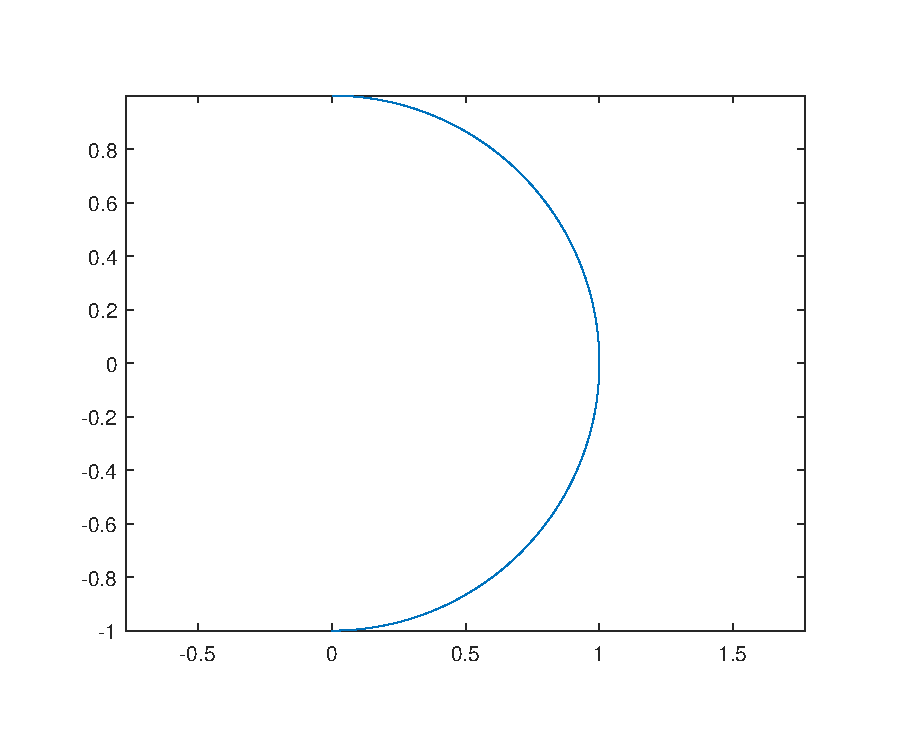
\includegraphics[width=10cm]{7b_1}
	\caption{$C = 1$}
\end{figure}

\begin{figure}[H]
	\centering	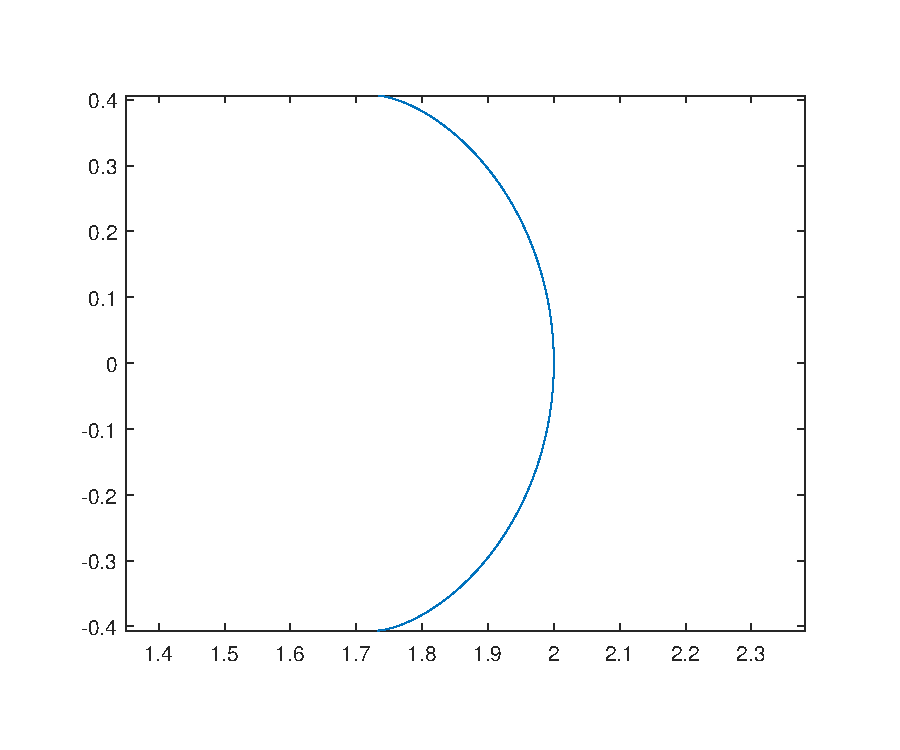
\includegraphics[width=10cm]{7b_g1}
	\caption{$C = 2$}
\end{figure}

\begin{figure}[H]
	\centering	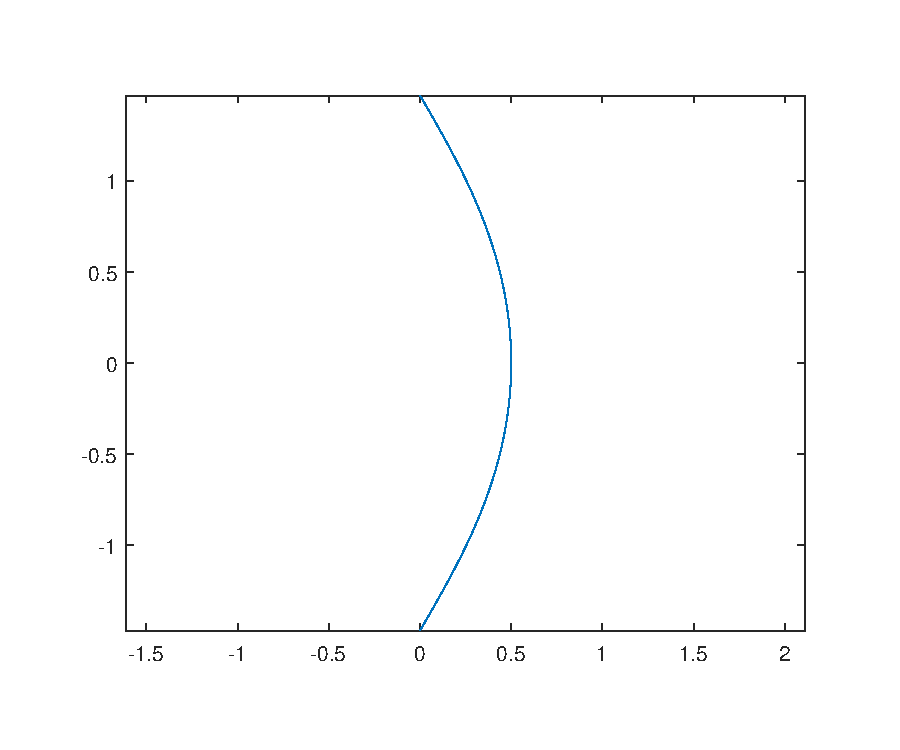
\includegraphics[width=10cm]{7b_l1}
	\caption{$C = \dfrac{1}{2}$}
\end{figure}

\newpage
\ref{7c} Recall the definition of some hyperbolic cosine and Hyperbolic sine
\begin{align}
\begin{cases}
\cosh v &= \dfrac{e^{v} + e^{-v}}{2}\\
\sinh v &= \dfrac{e^{v} - e^{-v}}{2}
\end{cases}
\end{align}
with the derivatives
\begin{align}
\begin{cases}
\cosh' v &= \dfrac{e^{v} - e^{-v}}{2} = \sinh v\\
\sinh' v &= \dfrac{e^{v} + e^{-v}}{2} = \cosh v
\end{cases}
\end{align}
If $K = -1$, using the result in \ref{7a}, we have the equation
\begin{align}
	\varphi'' - \varphi = 0 \label{7b_ode2}
\end{align}
This is a homogeneous second-order linear differential equation. The characteristic equation of \eqref{7b_ode2} is
\begin{align}
k^2 - 1 = 0 
\end{align}
The solutions of this characteristic equation are
\begin{align}
\begin{cases}
k_1 &= 1\\
k_2 &= -1
\end{cases}
\end{align} 
Hence, \eqref{7b_ode2} has the solution
\begin{align}
\varphi(v) = C_1 e^{v} + C_2 e^{-v} \label{7c_phi}
\end{align}
where $C_1$ and $C_2$ are arbitrary constants.

Differentiating $\varphi$ with respect to $v$, we have
\begin{align}
\varphi'(v) &= \left(C_1 e^{v} + C_2 e^{-v}\right)'\\
&= C_1 e^{v} - C_2 e^{-v} \label{7c_phi1}
\end{align}
Note that we have to specify the conditions for $C_1, C_2$ in order to determine the surfaces of revolution.

$\bullet$ \textbf{Case 1:} $C_1 = C_2 = \dfrac{C}{2}$
\begin{align}
\varphi(v) &= \frac{C}{2}( e^{v} + e^{-v})\\
&= C\frac{e^{v} + e^{-v}}{2}\\
&= C \cosh v \label{7c_phi_c1}\\
\varphi'(v) &= C \sinh v\\
\psi(v) &= \int_{0}^{v} \sqrt{1 - C^2 \sinh^2 \bar{v}}d\bar{v}
\end{align}
In order for \eqref{7a_psi} to makes sense,
\begin{align}
0 \leq C^2\sinh^2 v \leq 1
\end{align}
or
\begin{align}
\sinh^2 v \leq \frac{1}{C^2} 
\end{align}
or
\begin{align}
- \frac{1}{\lvert C\rvert}  \leq \sinh v \leq \frac{1}{\lvert C\rvert} 
\end{align}

\begin{figure}[H]
	\centering	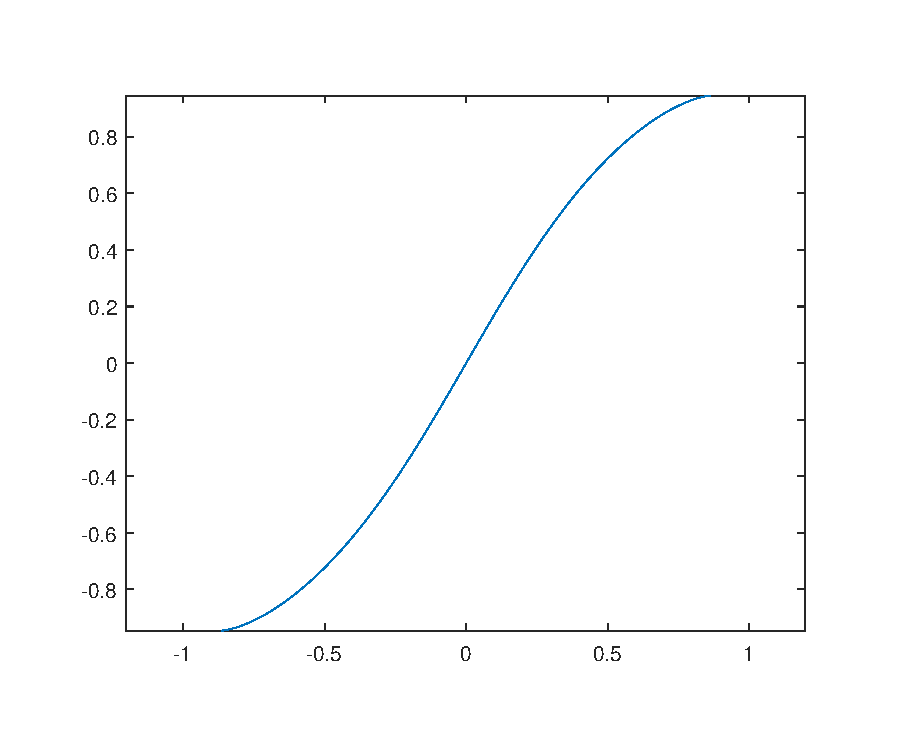
\includegraphics[width=10cm]{7c_1}
	\caption{Case 1, $C = 1$}
\end{figure}

$\bullet$ \textbf{Case 2:} $C_1 = \dfrac{C}{2}$ and $C_2 = -C_1 = \dfrac{C}{2}$
\begin{align}
\varphi(v) &= \frac{C}{2}( e^{v} - e^{-v})\\
&= C\frac{e^{v} - e^{-v}}{2}\\
&= C \sinh v \label{7c_phi_c2}\\
\varphi'(v) &= C \cosh v\\
\psi(v) &= \int_{0}^{v} \sqrt{1 - C^2 \cosh^2 \bar{v}}d\bar{v}
\end{align}
In order for \eqref{7a_psi} to makes sense,
\begin{align}
0 \leq C^2\cosh^2 v \leq 1
\end{align}
or
\begin{align}
\cosh^2 v \leq \frac{1}{C^2} 
\end{align}
or
\begin{align}
- \frac{1}{\lvert C\rvert}  \leq \cosh v \leq \frac{1}{\lvert C\rvert} 
\end{align}
%or
%\begin{align}
%- \arcosh \frac{1}{\lvert C\rvert}  \leq v \leq \arcosh \frac{1}{\lvert C\rvert} 
%\end{align}

\begin{figure}[H]
	\centering	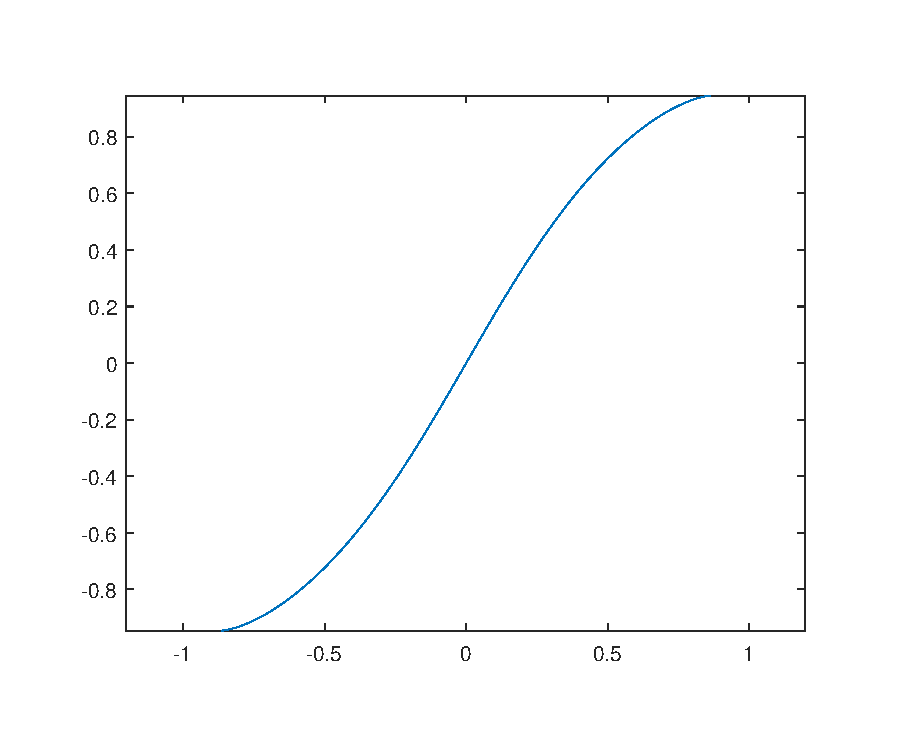
\includegraphics[width=10cm]{7c_2}
	\caption{Case 2, $C = 0.5$}
\end{figure}

$\bullet$ \textbf{Case 3:} $C_1 = 1$ and $C_2 = 0$
\begin{align}
\varphi(v) &= e^{v} \label{7c_phi_c3}\\
\varphi'(v) &= e^{v}\\
\psi(v) &= \int_{0}^{v} \sqrt{1 - e^{2} \bar{v}}d\bar{v}
\end{align}
In order for \eqref{7a_psi} to makes sense,
\begin{align}
0 \leq e^{2v} \leq 1
\end{align}
or
\begin{align}
e^{v} \leq 1
\end{align}
or
\begin{align}
v \leq 0
\end{align}

\begin{figure}[H]
	\centering	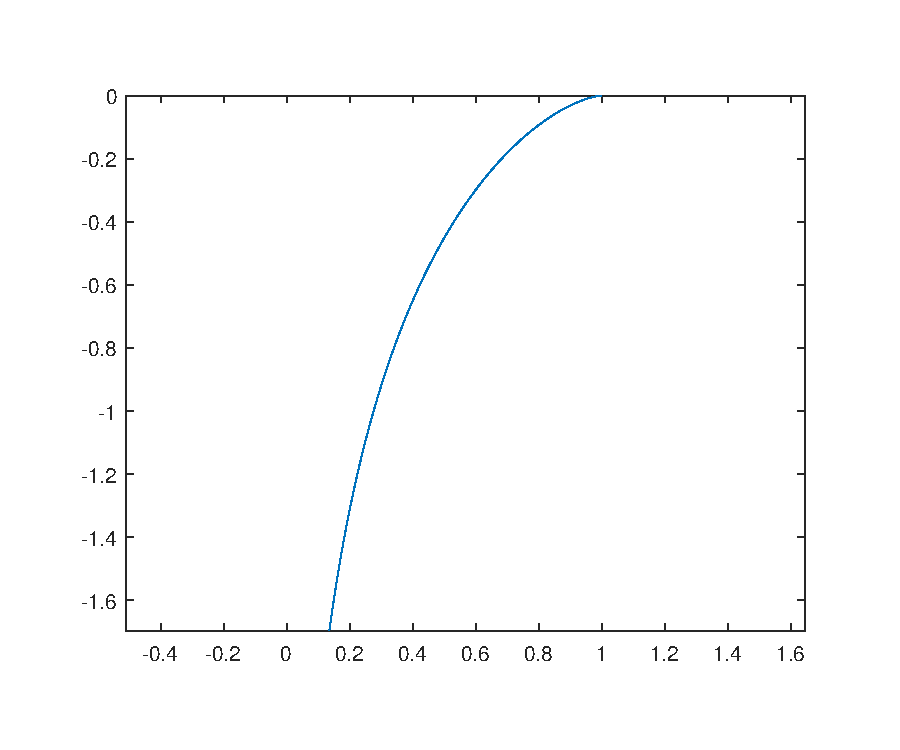
\includegraphics[width=10cm]{7c_3}
	\caption{Case 3}
\end{figure}
\newpage
\ref{7d} To check whether the surface of type 3 in \ref{7c} is the pseudosphere in \text{excercise 6}, we can check whether if the generating curve $(\varphi(v), \psi(v))$ in the plane $xOz$ is the tractrix as defined in \text{excercise 6}.

We have
\begin{align}
	\varphi(v) &= e^{v}\\
	\psi(v) &= \int_{0}^{v} \sqrt{1 - e^{2\bar{v} }}d\bar{v} 
\end{align}
The tangent vector of the generating curve $(\varphi(v), \psi(v))$ is
\begin{align}
(\varphi'(v), \psi'(v)) &= \left(e^{v},  \sqrt{1 - e^{2v }}\right)
\end{align}
Pick a point $\left(e^w, \int_{0}^{w} \sqrt{1 - e^{2\bar{w} }}d\bar{w} \right)$ on the generating curve ($w \in (0,1)$).

We are going to find the tangent line of the curve $(\varphi(v), \psi(v))$ at the point $\left(e^w, \int_{0}^{w} \sqrt{1 - e^{2\bar{w} }}d\bar{w} \right)$. We denote this tangent line as $T_w(x) = (x,ax + b)$ with $a$ and $b$ being unknown constants.

Since $T_w(x)$ go through $\left(e^w, \int_{0}^{w} \sqrt{1 - e^{2\bar{w} }}d\bar{w} \right)$, we have the equation
\begin{align}
	e^w a  + b = \int_{0}^{w} \sqrt{1 - e^{2\bar{w} }}d\bar{w} \label{7e_t1}
\end{align}
We also know that the tangent vector at $\left(e^w, \int_{0}^{w} \sqrt{1 - e^{2\bar{w} }}d\bar{w} \right)$ is
\begin{align}
	(\varphi'(w), \psi'(w)) &= \left(e^{w},  \sqrt{1 - e^{2w }}\right)
\end{align}
This implies that $T_w(x)$ must also go through the point
\begin{align}
	\left(e^w + e^{w}, \int_{0}^{w} \sqrt{1 - e^{2\bar{w} }}d\bar{w} + \sqrt{1 - e^{2w }} \right)  = \left(2e^w, \int_{0}^{w} \sqrt{1 - e^{2\bar{w} }}d\bar{w} + \sqrt{1 - e^{2w }} \right)
\end{align}
Thus, we have an other equation
\begin{align}
2 e^w a  + b = \int_{0}^{w} \sqrt{1 - e^{2\bar{w} }}d\bar{w} \sqrt{1 - e^{2w }}  \label{7e_t2}
\end{align}
We have the linear system of equation
\begin{align}
\begin{cases}
e^w a  + b &= \int_{0}^{w} \sqrt{1 - e^{2\bar{w} }}d\bar{w}\\
2 e^w a  + b &= \int_{0}^{w} \sqrt{1 - e^{2\bar{w} }}d\bar{w} + \sqrt{1 - e^{2w }} 
\end{cases}
\end{align}
Solve this system for $a$ and $b$, we obtain
\begin{align}
	&\begin{cases}
	a &= \dfrac{\int_{0}^{w} \sqrt{1 - e^{2\bar{w} }}d\bar{w} - \left(\int_{0}^{w} \sqrt{1 - e^{2\bar{w} }}d\bar{w} + \sqrt{1 - e^2w }\right)}{e^w - 2e^w}\\
	b &= \dfrac{e^w\left(\int_{0}^{w} \sqrt{1 - e^{2\bar{w} }}d\bar{w} + \sqrt{1 - e^{2w }}\right) - 2e^w\int_{0}^{w} \sqrt{1 - e^{2\bar{w} }}d\bar{w}}{e^w - 2e^w}
	\end{cases}\\
	\Longleftrightarrow\enskip&
	\begin{cases}
	a &= \dfrac{\sqrt{1 - e^2w }}{e^w}\\
	b &= \int_{0}^{w} \sqrt{1 - e^{2\bar{w} }}d\bar{w} - \sqrt{1 - e^{2w }}
	\end{cases}
\end{align}
Hence, we can find that the intersection of the tangent line of the generating curve at $\left(e^w, \int_{0}^{w} \sqrt{1 - e^{2\bar{w} }}d\bar{w} \right)$ and the z-axis is
\begin{align}
	\left(0,b\right) = \left(0, \int_{0}^{w} \sqrt{1 - e^{2\bar{w} }}d\bar{w} - \sqrt{1 - e^{2w }}\right)
\end{align}
The distance between $\left(e^w, \int_{0}^{w} \sqrt{1 - e^{2\bar{w} }}d\bar{w} \right)$ and $\left(0, \int_{0}^{w} \sqrt{1 - e^{2\bar{w} }}d\bar{w} - \sqrt{1 - e^{2w }}\right)$ is
\begin{align}
	&\sqrt{\left(0 - e^w\right)^2 + \left(\int_{0}^{w} \sqrt{1 - e^{2\bar{w} }}d\bar{w} - \sqrt{1 - e^{2w }} - \int_{0}^{w} \sqrt{1 - e^{2\bar{w} }}d\bar{w}  \right)^2}\\ =& \sqrt{\left(e^w\right)^2 + \left(\sqrt{1 - e^{2w }}\right)^2}\\
	=& \sqrt{e^{2w} + 1 - e^{2w }}\\
	=& 1
\end{align}
Therefore, the generating curve $(\varphi(v), \psi(v))$ is a tractrix and the surface of revolution it generates is a pseudosphere.

\newpage
\ref{7e} 
If $K = 0$, using the result in \ref{7a}, we have the equation
\begin{align}
\varphi''  = 0 \label{7e_ode1}
\end{align}
This is a homogeneous second-order linear differential equation. The characteristic equation of \eqref{7e_ode1} is
\begin{align}
k^2  = 0 
\end{align}
The solution of this characteristic equation is
\begin{align}
\begin{cases}
k = 0
\end{cases}
\end{align} 
Hence, \eqref{7e_ode1} has the solution
\begin{align}
\varphi(v) &= e^{0v} (C_1  + C_2v)\\
 &= C_1  + C_2v \label{7e_phi}
\end{align}
where $C_1$ and $C_2$ are arbitrary constants.

We also have
\begin{align}
\varphi'(v) &= (C_1  + C_2v)'\\
&= C_2
\end{align}
and
\begin{align}
	\psi(v) &= \int_{0}^{v} \sqrt{1 - {\varphi'}^2(\bar{v})} d\bar{v}\\
	&= \int_{0}^{v} \sqrt{1 - C_2^2} d\bar{v}\\
	&= v\sqrt{1 - C_2^2}
\end{align}
where $-1\leq C_2\leq 1$

$\bullet$ \textbf{Case 1:} $C_2 = 1$ or $C_2 = -1$ 

In this case, the generating curve is
\begin{align}
(\varphi(v),\psi(v)) &= \left(C_1 + C_2 v,v\sqrt{1 - C_2^2}\right)\\
&= \left(C_1 + C_2 v,0\right)
\end{align}
which is a line orthogonal to the z-axis.

Therefore, the surface of revolution in this case is a plane.

$\bullet$ \textbf{Case 2:} $C_2 = 0$

In this case, the generating curve is
\begin{align}
(\varphi(v),\psi(v)) &= \left(C_1,v\sqrt{1 - 0^2}\right)\\
&= \left(C_1,v\right)
\end{align}
which is a line orthogonal to the x-axis.

Therefore, the surface of revolution in this case is a right circular cylinder.

$\bullet$ \textbf{Case 3:} $C_1 \neq 0$ and $0 < \lvert C_2\rvert < 1$ 

In this case, the generating curve is
\begin{align}
(\varphi(v),\psi(v)) &= \left(C_1 + C_2 v,v\sqrt{1 - C_2^2}\right)
\end{align}
which is a line x-axis and it intersect the z-axis at $\left(0, -\frac{C_1\sqrt{1 - C_2^2}}{C_2}\right)$.

Therefore, the surface of revolution in this case is a right circular cone.

\newpage
\printindex
\newpage
\begin{thebibliography}{999}
\bibitem [DG\_Kunnel]{1} Wolfgang Kunnel, \textit{Differential Geometry: Curves, Surfaces, Manifolds}, 2nd edition, AMS, 2006.
\bibitem [DG\_Carmo\_1]{2} Manfredo P. Do Carmo, \textit{Differential Geometry of Curves and Surfaces}, 1st edition, Prentice-Hall, 1976.
\end{thebibliography}
\end{document}